\documentclass[border=10pt]{standalone}

\usepackage{tikz}
\usepackage{tikzsymbols}
\usetikzlibrary{calc,patterns,shapes.geometric}

\def\centerarc[#1](#2)(#3:#4:#5){\draw[#1] ($(#2)+({#5*cos(#3)},{#5*sin(#3)})$) arc (#3:#4:#5);}

\begin{document}
	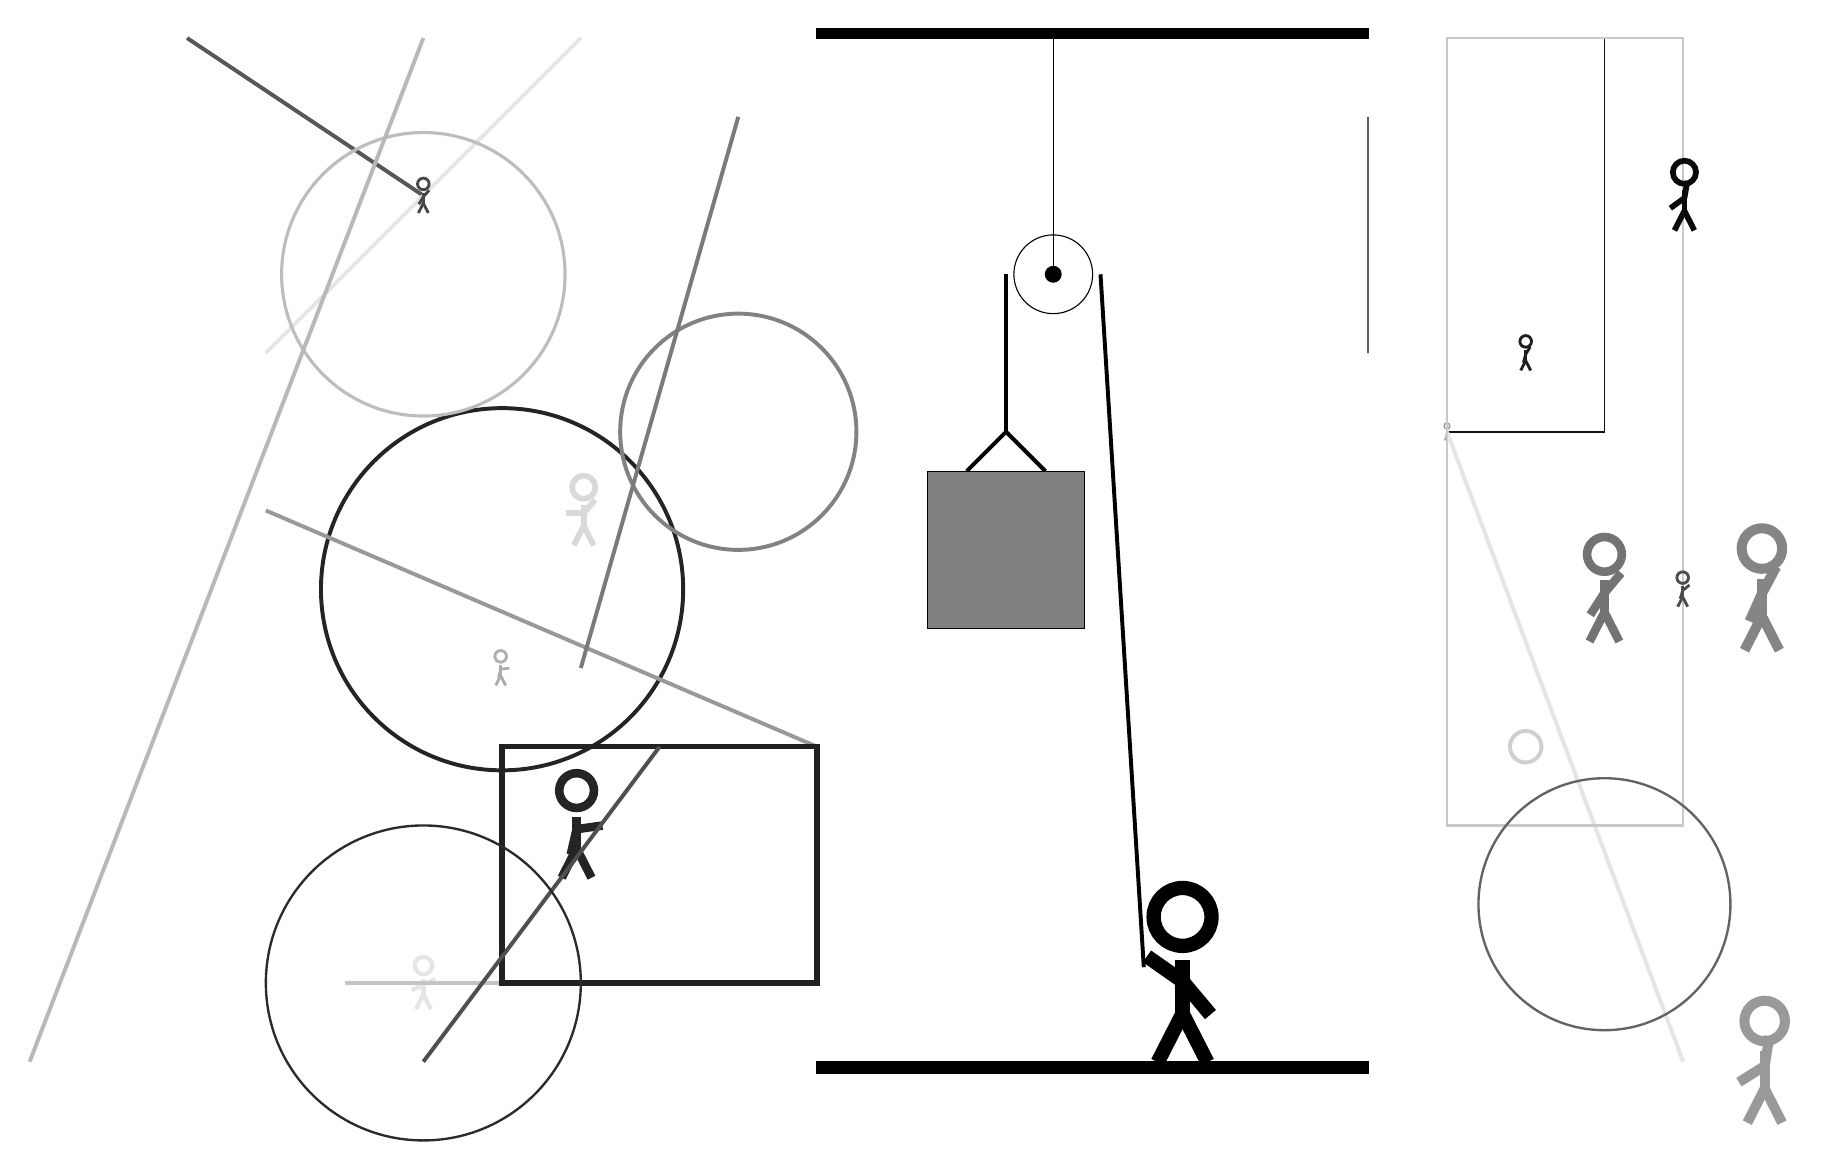
\begin{tikzpicture}
		%%%%% START %%%%%
		
		\draw[fill=black] (-2, 10) rectangle (5, 10.125);
		
		\draw (1, 7) circle (0.5);
		\draw[fill=black] (1, 7) circle (0.1);
		\draw (1, 10) -- (1, 7);
		
		\draw[line width=0.5mm] (-0.1, 4.5) -- (0.4, 5.0) -- (0.9, 4.5);
		\draw[fill=black!50] (-0.6, 4.5) rectangle (1.4, 2.5);
		
		\node[line width=0.4mm, color=black!39] at (6, 5) {\Strichmaxerl[1][75][82]};
		
		\node[line width=0.2mm, color=black!15] at (-5, 4) {\Strichmaxerl[4][0][49]};
		\node[line width=0.7mm, color=black!10] at (-7, -2) {\Strichmaxerl[3][25][27]};
		\draw [line width=0.5mm, color=black!86](-6, 3) circle (2.3);
		\draw[line width=0.5mm, color=black!66](-7, 8) -- (-10, 10);
		\node[line width=0.2mm, color=black!88] at (7, 6) {\Strichmaxerl[2][75][59]};
		\draw[line width=0.5mm, color=black!10](-5, 10) -- (-9, 6);
		
		\node[line width=0.7mm, color=black!40] at (10, -3) {\Strichmaxerl[7][32][81]};
		\node[line width=0.7mm, color=black!72] at (-7, 8) {\Strichmaxerl[2][59][48]};
		\draw[line width=0.5mm, color=black!23](-5, -2) -- (-8, -2);
		
		\draw [line width=0.5mm, color=black!19](7, 1) circle (0.2);
		
		\draw[line width=0.5mm, color=black!40](-2, 1) -- (-9, 4);
		\draw[line width=0.2mm, color=black!93] (6, 5) rectangle (8, 10);
		
		\draw[line width=0.5mm, color=black!10](6, 5) -- (9, -3);
		\draw[line width=0.3mm, color=black!21] (6, 0) rectangle (9, 10);
		\draw [line width=0.5mm, color=black!49](-3, 5) circle (1.5);
		
		\node[line width=0.7mm, color=black!86] at (-5, 0) {\Strichmaxerl[6][77][8]};
		
		\draw[line width=0.3mm, color=black!62] (5, 9) rectangle (5, 6);
		\draw[line width=0.7mm, color=black!87] (-2, 1) rectangle (-6, -2);
		\draw[line width=0.5mm, color=black!69](-7, -3) -- (-4, 1);
		\node[line width=0.3mm, color=black!48] at (10, 3) {\Strichmaxerl[7][66][62]};
		
		\node[line width=0.7mm, color=black!70] at (9, 3) {\Strichmaxerl[2][73][39]};
		\draw [line width=0.4mm, color=black!26](-7, 7) circle (1.8);
		\node[line width=0.3mm, color=black!32] at (-6, 2) {\Strichmaxerl[2][76][7]};
		\node[line width=0.5mm, color=black!55] at (8, 3) {\Strichmaxerl[6][57][50]};
		\node[line width=0.4mm, color=black!96] at (9, 8) {\Strichmaxerl[4][36][80]};
		\draw [line width=0.3mm, color=black!61](8, -1) circle (1.6);
		\draw [line width=0.3mm, color=black!83](-7, -2) circle (2.0);
		
		\draw[line width=0.5mm, color=black!28](-7, 10) -- (-12, -3);
		
		\draw[line width=0.5mm, color=black!52](-5, 2) -- (-3, 9);
		
		\draw[line width=0.5mm] (0.4, 7) -- (0.4, 5.0);
		\centerarc[line width=0.5mm](1, 7)(0:180:0.6);
		\draw[line width=0.5mm](1.6, 7) -- (2.15, -1.8);
		
		\node at (2.6, -1.9) {\Strichmaxerl[10][-35][-50]};
		
		\draw[fill=black] (-2, -3) rectangle (5, -3.15);
		
		%%%%% END %%%%%
	\end{tikzpicture}
\end{document}